\newpage
\begin{center}
  \textbf{\large 3. Эксперименты}
\end{center}
\refstepcounter{chapter}
\addcontentsline{toc}{chapter}{3. Эксперименты}

В данном разделе приведено описание экспериментов. Для проверки работы разработанного метода были выбраны 2 манипуляционные задачи: открытие шкафа и взятие банки. Для первой задачи эксперименты были проведены в симуляторе для одной модели, в результате была проведена оценка робастности исследуемой модели и определены наиболее значимые компоненты среды, к которым модель особенно чувствительна. Для второй задачи эксперименты были проведены в симуляторе для трёх моделей, также была рассчитана корреляция полученных метрик с эффективностью моделей в реальности. 

\section{Задача открытия шкафа}

    \subsection{Описание среды}

        Манипулятору требуется открыть выдвижной ящик шкафа на заданное расстояние. В качестве наблюдений доступно следующее:

        \begin{itemize}
            \item Изображение с камеры $I$, расположенной на инструменте робота;
            \item Информация о положениях сочленений робота $q$;
            \item Информация о скоростях сочленений робота $\dot{q}$.
        \end{itemize}

        Манипулятором является 7-ми осевой робот Franka Emika Panda. Эпизод считается успешным, если агент менее, чем за 800 итераций, открывает выдвижной ящик на 15 сантиметров от исходного положения, изначально шкаф закрыт. 
        
        В начале каждого эпизода, рандомизируются положение и ориентация шкафа, а также начальное положение сочленений робота. 

    \subsection{Процесс обучения}

        Для обучения агента был использован алгоритм имитационного обучения, а именно клонирование поведения. Для обработки изображений извлекались признаки с помощью нейросетевой архитектуры ResNet18 \cite{he2015deepresiduallearningimage}. Веса модели были взяты из фреймворка IsaacLab и заморожены. 
        
        Было записано 1000 успешных экспертных демонстраций, каждая демонстрация содержала следующую информацию:~\begin{itemize}
            \item Признаки изображения $f(I)$;
            \item Информация о положениях сочленений робота $q$;
            \item Информация о скоростях сочленений робота $\dot{q}$.
        \end{itemize}

        Хранение в демонстрациях не исходных изображений, а их признаков позволяет значительно уменьшить размер обучающего набора данных, снизить размер итоговой модели и заметно уменьшить время обучения. 

        Обучение проводилось на 2000 эпохах и заняло приблизительно 60 минут с использованием видеокарты NVIDIA GeForce RTX 4070 16 GB. По итогу обучения, на исходной среде доля успешных эпизодов агента составила примерно: $R_0 = 0.7$.

        \subsection{Результаты экспериментов}

            Согласно пункту \ref{method} была проведена валидация обученной модели на различных вариациях среды, результаты представлены на таблице \ref{res-Table1}. Для каждой вариации эксперимент проводился на 50 эпизодах ($N = 50$). Параметры вариаций представлены в \hyperref[sec:results]{приложении А}.

            \begin{table}[h]
              \caption{Результаты валидации модели BC на задаче с отрытием шкафа}
              \label{res-Table1}
              \centering{
                \begin{tabular}{ |c|c|c| }
                  \hline
                  Рандомизация & $R_j$ & $\Delta R_j$ \\ \hline 
                 Исходная среда & 0.7 & - \\ \hline
                 \multicolumn{3}{|c|}{\textit{Визуальные параметры}} \\ \hline  
                 Текстура ОМ & 0.0 & 0.7 \\ \hline
                 Цвет ОМ & 0.04 & 0.66 \\ \hline
                 Текстура заднего плана & 0.54 & 0.16 \\ \hline
                 Цвет заднего плана & 0.3 & 0.4 \\ \hline
                 Цвет источника освещения & 0.72 & 0.02 \\ \hline
                 Отвлекающий объект & 0.5 & 0.2 \\ \hline
                 Смещение камеры & 0.56 & 0.14 \\ \hline
                  \multicolumn{3}{|c|}{\textit{Физические параметры}} \\ \hline  
                   Масса объектов & 0.62 & 0.08 \\ \hline 
                   Трения объектов & 0.34 & 0.36 \\ \hline
                   \multicolumn{2}{|c|}{\textbf{Оценка робастности $\Delta R$:}} & \textbf{0.3} \\ \hline
                \end{tabular}
              }
              
            \end{table}

            По результатам исследуемая модель оказывается достаточно чувствительной к визуальным компонентам среды, особенно к внешнему виду объекту манипулирования. Также модель уязвима к коэффициентам трения объекта манипулирования. Подобные результаты оценки робастности можно объяснить плохой обобщающей способностью, присущей моделям имитационного обучения. 

    \section{Задача взятия банки}

        \subsection{Описание среды}

            Манипулятору требуется поднять алюминиевую банку, стоящую на столе. В качестве наблюдений доступно следующее:

            \begin{itemize}
                \item Изображение с камеры $I$, расположенной на теле робота;
                \item Языковая инструкция.
            \end{itemize}

            Манипулятором является робот Google Robot. Эпизод считается успешным, если агент поднял банку не менее чем на 4 см над столом. 
            
            В начале каждого эпизода, рандомизируются положение банки, а также начальное положение сочленений робота. 

        \subsection{Процесс обучения}

            В качестве исследуемых агентов взяты 3 модели на основе архитектуры RT-1 \cite{brohan2023rt1roboticstransformerrealworld}:

            \begin{enumerate}
                \item RT-1 $(100\%)$ -- полностью обученная модель;
                \item RT-1 $(15\%)$ -- модель после $15\%$ обучающих итераций;
                \item RT-1 $(0\%)$ -- модель в начале обучения.
            \end{enumerate}
            
            Веса моделей, как и среда взяты из работы Simpler \cite{li24simpler}, где также подробно описан процесс обучения. Так как данные модели были обучены на реальных данных, необходимо воссоздать аналогичную среду в симуляторе, которая будет считаться исходной. 

        \subsection{Результаты экспериментов}

            Согласно пункту \ref{method} была проведена валидация и рассчитана корреляция обученных моделей на различных вариациях среды, результаты представлены на таблице \ref{res-Table2}. Для каждой вариации эксперимент проводился на 10 эпизодах ($N = 10$). Параметры вариаций представлены в \hyperref[sec:results]{приложении А}.

            \begin{table}[h]
              \caption{Результаты валидации моделей RT-1 на задаче взятия банки}
              \label{res-Table2}
              \centering{
                \begin{tabular}{ |c|c|c|c|c|c|c| }
                  \hline
                  Модель & \multicolumn{2}{|c|}{RT-1 $(100\%)$} & \multicolumn{2}{|c|}{RT-1 $(15\%)$} & \multicolumn{2}{|c|}{RT-1 $(0\%)$} \\ \hline
                  Рандомизация &  $R_j$ & $\Delta R_j$ &  $R_j$ & $\Delta R_j$ &  $R_j$ & $\Delta R_j$ \\ \hline 
                 Исходная среда & 0.8 & - & 0.5 & - & 0.2 & - \\ \hline
                 \multicolumn{7}{|c|}{\textit{Визуальные параметры}} \\ \hline  
                 Текстура ОМ & 0.5 & 0.3 & 0.5 & 0.0 & 0.3 & 0.1 \\ \hline
                 Цвет ОМ & 0.6 & 0.2 & 0.3 & 0.2 & 0.2 & 0.0 \\ \hline
                 Текстура заднего плана & 0.5 & 0.3 & 0.6 & 0.1 & 0.1 & 0.1 \\ \hline
                 Цвет заднего плана & 0.8 & 0.0  & 0.5 & 0.0  & 0.2 & 0.0 \\ \hline
                 Цвет источника освещения & 0.7 & 0.1 & 0.6 & 0.1 & 0.2 & 0.0 \\ \hline
                 Отвлекающий объект & 0.8 & 0.20& 0.5 & 0.0 & 0.1 & 0.1 \\ \hline
                 Смещение камеры & 0.8 & 0.0 & 0.4 & 0.1 & 0.3 & 0.1 \\ \hline
                  \multicolumn{7}{|c|}{\textit{Физические параметры}} \\ \hline  
                   Масса объектов & 0.8 & 0.0 & 0.8 & 0.3 & 0.2 & 0.0 \\ \hline 
                   Трения объектов & 0.7 & 0.1 & 0.4 & 0.1 & 0.3 & 0.1 \\ \hline \hline
                   \textbf{Среднее значение:} & \textbf{0.69} & \textbf{0.12} & \textbf{0.51} & \textbf{0.1} & \textbf{0.21} & \textbf{0.06} \\ \hline
                \end{tabular}
              }
              
            \end{table}

            По результатам эксперимента можно сделать вывод, что данные модели имеют хорошую обобщающую способность и достаточно робастны по всем параметрам. Однако подобный вывод невозможно сделать о модели RT-1 $(0\%)$, эффективность которой мала как на исходной среде, так и на вариациях. Из этого эксперимента следует, что оценка робастности валидна, только если агент имеет достаточную эффективность на исходной среде. Также большую роль играет исходная среда, как указано выше, исходная среда была воссоздана на основе реальной, поэтому результаты оценки робастности сильно зависят от качества этой среды.

            Также была рассчитана корреляция доли успешных эпизодов по всем вариациям с эффективностью модели в реальности. Данные о результатах в реальности взяты из работы Simpler. Полученный коэффициент корреляции Пирсона составил $r = 0.897$. Высокий показатель говорит о том, что данный метод можно использовать для прогнозирования эффективности модели в реальных условиях, посредством валидации на вариациях. Визуализация результатов представлена на рис. (\ref{fig:res})

            \begin{figure}
              \begin{center}
                  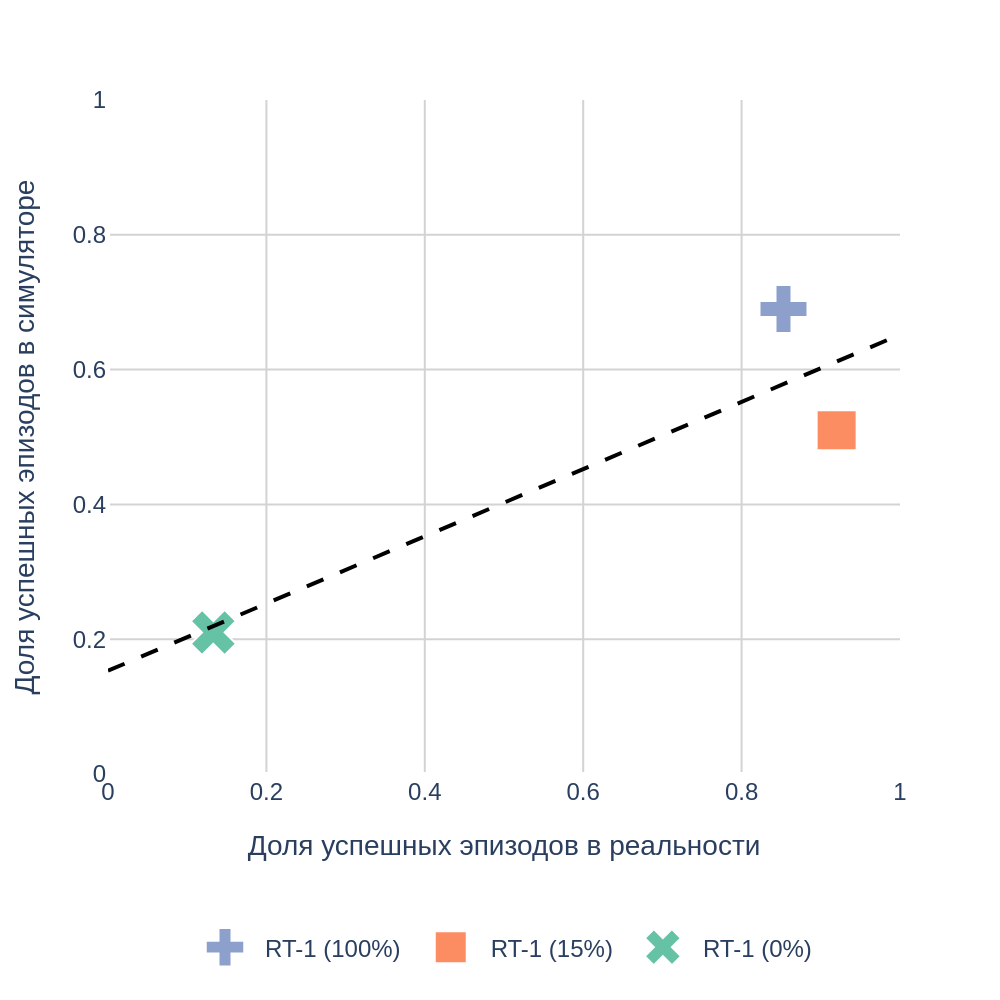
\includegraphics[width=0.6\textwidth]{images/plot.png}
              \caption{Сравнение эффективности моделей в реальности и в симуляторе}
              \label{fig:res}
              \end{center}
          \end{figure}